% Chapter 12 of Volume III: Kernels, splines and Hankel ladders: two candidate mechanisms. Sources: misc/reviews/nick-volume3/vol3/ch5_candidates.tex (lines per misc/vol3/STRUCTURE.md, Chapter 12); reports U05 M1 to M12 (misc/research/directions/opus/vol3/U05.md) and referee_candidates.md (V3D); verification W2 (V5, V6, V18) and W5 (V7); 17 Nov 2026.
\label{c:ch:cand}

Chapter~\ref{p:ch:path} reduced RH to one statement: the Riemann density $F$, the law with characteristic function $\xi(\frac12)/\xi(\frac12+\tau)$ at real $\tau$, is a P\'olya frequency function. It showed that a finite set of rungs detects no zero below the verified height, and asked for a mechanism, a construction from the primes and the gamma function that makes total positivity visible. Two candidates were named. The first is Jackson's $q$ Gamma function: it writes $\Gamma(s/2)$ as a limit of products of Euler factors at a fake prime $P\downarrow1$, each factor has a total positivity property, and the hope was that the product inherits it. The second is the B spline of Curry and Schoenberg: every P\'olya frequency function is a limit of B splines, the knots of $F$ are the reciprocal zeros, and the hope was to define the knots from prime data. A mechanism that cannot tell $\zeta$ from the Davenport and Heilbronn control cannot prove RH, and this chapter works both candidates through against that test. The kernel, knot and ladder computations are from an unrefereed note of Polson (November 2026) and were recomputed here where stated. The outcome is negative for both in their naive form, and the reasons are precise.

The Euler factors are totally positive on their own lattices and not on the line. The total positivity they generate lives on the kernel side, in Riemann's kernel $\Phi$, and stops at a finite rung: $\Phi$ is totally positive of order $4$ and not of order $5$ (computed in floating point, not certified). The kernel ladder does not see the zeros: the control fails at rung $3$, and so does the Dirichlet $L$ function modulo $4$ (Section~\ref{c:sec:kernel}). Knots built from the gamma factor alone approximate $F$ to $0.4$ per cent and the control's density to $1.2$ per cent, so they do not separate the two. Knots corrected by primes locate the zeros on average, but at a fixed low height they stop moving once the cutoff passes a finite value, and the construction that does converge, to the ordinates of the zeros, converges whether or not the zeros are on the line. The step that remains is an identity between two functions that differ, for the control, by $8$ parts in $10^8$ (Section~\ref{c:sec:knots}). The crossing from $\xi$ to $1/\xi$ exists, and it is not total positivity of the kernel: it is the Wald couple of Roynette and Yor, equivalently a van Dantzig pair, and RH says that the mixing variable is a generalised gamma convolution (Section~\ref{c:sec:wald}). The kernels of that section have first failing orders of total positivity from $3$ to never, so the order of the kernel carries no information about the zeros. The positivity of the Thorin measure has its own ladder of Hankel determinants, computable from the Taylor coefficients of $\log\xi$ at $\frac12$; $\zeta$ passes its first $50$ rungs and so does the control, which makes it a blunter test than the ladder of $F$ (Section~\ref{c:sec:grommer}). Section~\ref{c:sec:verdict} states what a mechanism must look like after these findings. Unless a proof is given or a source cited, numerical statements are computed in floating point, and ``certified'' is not used: the verification of this chapter did not run interval arithmetic.

\section{Two sides: the kernel and the density}\label{c:sec:sides}

Riemann's kernel is the function $\Phi$ of Section~\ref{ch:clock}, in Titchmarsh's normalisation,
\[
\Phi(u)=2\sum_{n\ge1}\big(2\pi^2n^4e^{9u/2}-3\pi n^2e^{5u/2}\big)e^{-\pi n^2e^{2u}},
\]
a positive even function with
\begin{equation}\label{c:eq:kernel}
\int_{\mathbb R}\Phi(u)e^{tu}\,\mathrm{d}u=\xi(\tfrac12+t),\qquad \xi(s)=\tfrac12s(s-1)\pi^{-s/2}\Gamma(s/2)\zeta(s).
\end{equation}
The density $F$ sits on the other side: its characteristic function at real $\tau$ is the reciprocal $\xi(\frac12)/\xi(\frac12+\tau)$. The same real axis data appear twice, once as the Laplace transform of $\Phi$ and once, inverted, as the Fourier transform of $F$.
\begin{center}
\footnotesize
\begin{tabular}{lll}
\toprule
 & kernel side & density side\\
\midrule
function & $\Phi$ & $F$\\
transform & $\xi(\frac12+t)$ & $\xi(\frac12)/\xi(\frac12+\tau)$\\
built from & gamma kernel, prime lattices & zeros\\
PF of all orders & never (Proposition~\ref{c:prop:gauss}) & if and only if RH\\
\bottomrule
\end{tabular}
\end{center}

\begin{proposition}\label{c:prop:gauss}
Let $K$ be a positive integrable function whose two sided Laplace transform $M(t)=\int K(u)e^{tu}\,\mathrm{d}u$ is entire. If $K$ is a P\'olya frequency function, then $K$ is a Gaussian. In particular $\Phi$, and the kernel of every $L$ function with an entire completed form and zeros, fails some rung PF$_k$.
\end{proposition}

\begin{proof}
By Schoenberg's theorem \cite{Schoenberg51} the transform of an integrable P\'olya frequency function is $1/\Psi$ on its strip, with $\Psi(t)=Ce^{-ct^2+bt}\prod(1+a_\nu t)e^{-a_\nu t}$, $c\ge0$, $a_\nu$ real, $\sum a_\nu^2<\infty$. If $M=1/\Psi$ is entire then $\Psi$ has no zeros, so $M(t)=C^{-1}e^{ct^2-bt}$ and $K$ is a Gaussian. The transform \eqref{c:eq:kernel} has zeros, so $\Phi$ is not of this form.
\end{proof}

Total positivity of all orders can hold on the density side only. On the kernel side the ladder must break, and the questions are where it breaks and whether the place carries information about the zeros.

\section{Candidate one: the fake prime and the kernel side}\label{c:sec:kernel}

\subsection{What an Euler factor is totally positive for}

The Euler factor of a prime $p$ is $(1-p^{-s})^{-1}=\sum_{m\ge0}p^{-ms}$, the Laplace transform of the measure $\mu_p=\sum_{m\ge0}\delta_{m\log p}$.

\begin{proposition}\label{c:prop:lattice}
The sequence of weights of $\mu_p$ is a P\'olya frequency sequence on the lattice $\mathbb Z\log p$. As a kernel on the line, $\mu_p$ is not totally positive of order two.
\end{proposition}

\begin{proof}
A geometric sequence has generating function $1/(1-z)$, which is of Edrei's form \cite{Edrei53}, so it is a P\'olya frequency sequence. On the line put $h=\log p$ and take $x_1=\frac h2$, $x_2=h$, $y_1=0$, $y_2=\frac h2$. Then $\mu_p\{x_1-y_1\}=\mu_p\{x_2-y_2\}=0$, because $\frac h2$ is not a lattice point, while $\mu_p\{x_1-y_2\}=\mu_p\{x_2-y_1\}=1$. The $2\times2$ minor equals $-1$.
\end{proof}

\subsection{Jackson's function}

For $0<q<1$,
\[
\Gamma_q(x)=(1-q)^{1-x}\prod_{k\ge0}\frac{1-q^{k+1}}{1-q^{k+x}}=\sum_{k\ge0}w_k\,e^{-xu_k},
\]
with $u_k=k|\log q|+\log(1-q)$ and $w_k=(1-q)(q;q)_\infty/(q;q)_k$, by Euler's identity $\prod_{k\ge0}(1-q^kz)^{-1}=\sum_kz^k/(q;q)_k$. With $q=P^{-2}$ the product is a product of Euler factors of the fake prime $P$ at the shifts $s,s+2,s+4,\dots$ (Chapter~\ref{g:ch:gammaprimes}).

\begin{proposition}\label{c:prop:jackson}
For every $0<q<1$ the weights $w_k$ form a P\'olya frequency sequence, and the measure $\sum w_k\delta_{u_k}$ is not totally positive of order two on the line. As $q\uparrow1$ the measure converges vaguely to $\exp(-e^{-u})\,\mathrm{d}u$, the kernel of $\Gamma(x)=\int e^{-xu}\exp(-e^{-u})\,\mathrm{d}u$, whose integrable tilts $e^{-au}\exp(-e^{-u})$, $a>0$, are P\'olya frequency functions.
\end{proposition}

\begin{proof}
The generating function $\sum_kz^k/(q;q)_k=\prod_k(1-q^kz)^{-1}$ is of Edrei's form. The failure on the line is as in Proposition~\ref{c:prop:lattice}. The limit is the convergence $\Gamma_q\to\Gamma$ of Laplace transforms. The tilted limit kernel is a P\'olya frequency function because $1/\Gamma$ is entire with real zeros $0,-1,-2,\dots$ and genus one.
\end{proof}

Figure~\ref{c:fig:qkernel} (left) compares the weights per unit length, $w_k/|\log q|$, with the limit. The supremum over the lattice of the difference is the limit $k\to\infty$, equal to $1-(1-q)/|\log q|$, which is $0.28$, $0.10$ and $0.025$ for $q=0.5$, $0.8$ and $0.95$ (computed): the discrepancy sits in the tail, not in the bulk. So total positivity on the line, in the tilted sense, is a property of the limit $P\downarrow1$ only. The fake prime acquires it because its lattice becomes dense. A real prime never does.

\begin{figure}[t]
\centering
% The left panel plots w_k/|log q| against exp(-e^{-u}); numbers confirmed by the verification (V18). The right panel shows the first failing rung of Table c:tab:kernel (V5), confirmed.
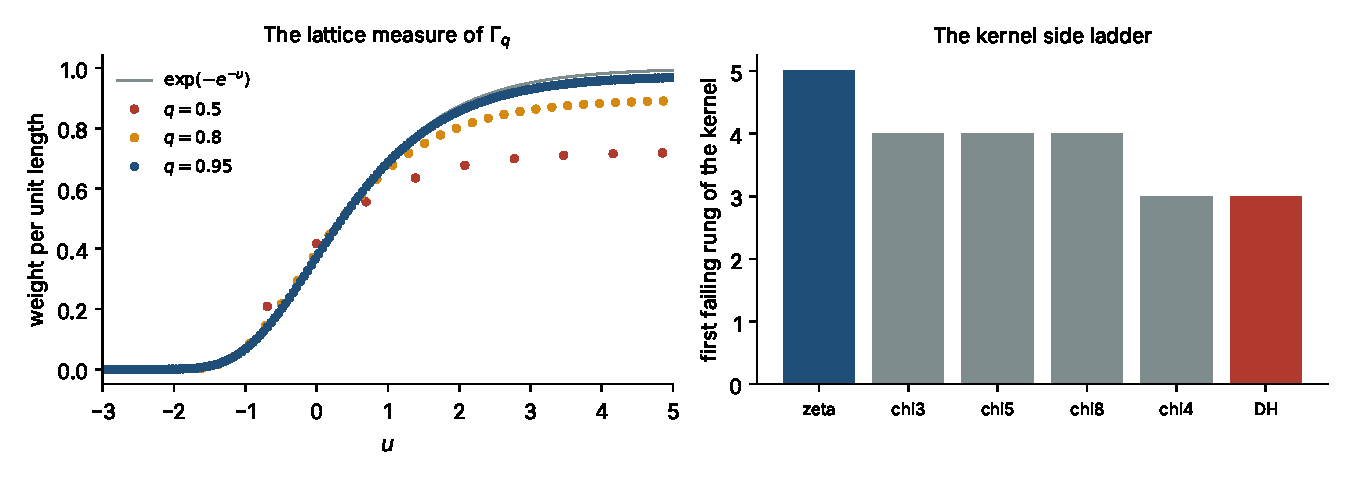
\includegraphics[width=\textwidth]{fig/v3/fig_qkernel.pdf}
\caption{Left: the lattice measure of Jackson's $\Gamma_q$, as weight per unit length, against the kernel $\exp(-e^{-u})$ of $\Gamma$. Right: the first failing rung of the kernel for $\zeta$, for four Dirichlet $L$ functions and for the Davenport and Heilbronn control.}
\label{c:fig:qkernel}
\end{figure}

\subsection{The kernel is the product, and its ladder is short}

Put $g(u)=2(2\pi^2e^{9u/2}-3\pi e^{5u/2})e^{-\pi e^{2u}}$. Then
\[
\Phi(u)=\sum_{n\ge1}n^{-1/2}\,g(u+\log n),
\]
the summand $g$ convolved with the product over primes of the lattice measures $\sum_mp^{-m/2}\delta_{-m\log p}$, and $\int g(u)e^{tu}\,\mathrm{d}u=\frac12s(s-1)\pi^{-s/2}\Gamma(s/2)$ at $s=\frac12+t$. This is the sense in which the completed zeta function is a product of Euler factors, one of them at the fake prime in the limit. Only the factor $\pi^{-s/2}\Gamma(s/2)$, the transform of the positive kernel $2e^{u/2}e^{-\pi e^{2u}}$, is totally positive. The factor $\frac12s(s-1)$ is a differential operator, and $g$ itself is negative for $u<\frac12\log\frac3{2\pi}=-0.37$, so it fails even total positivity of order one. The lattices of the primes are incommensurable, and Proposition~\ref{c:prop:gauss} shows that the product cannot be totally positive of every order. We computed how far it gets.

We compare with the kernels of four real primitive characters and of the control. For a real primitive character $\chi$ modulo $q$ of parity $a\in\{0,1\}$ ($a=0$ for $\chi(-1)=1$) the kernel of the completed $L$ function is, up to a constant,
\[
K_\chi(u)=e^{(a+1/2)u}\sum_{n\ge1}\chi(n)n^a\exp\big(-\pi n^2e^{2u}/q\big).
\]
We took the odd characters modulo $3$ and $4$ and the even characters modulo $5$ and $8$ (there are two real primitive characters modulo $8$, and ours is the even one). The control is the Davenport and Heilbronn function $f(s)=\sum_n\psi(n)n^{-s}$ of Section~\ref{sec:ch21:hankel}, with $\psi=\re\chi+\kappa\,\im\chi$, $\chi$ an odd character of order $4$ modulo $5$ and $\kappa=0.284079$, so that $\xi_f(s)=(5/\pi)^{s/2}\Gamma(\frac{s+1}2)f(s)$ and the kernel is $K_f(u)=e^{3u/2}\sum_n\psi(n)n\exp(-\pi n^2e^{2u}/5)$ \cite{DH36}.

A search over $1.5\times10^5$ to $3\times10^5$ random minors $\det[K(x_i-y_j)]$ of orders $3$, $4$ and $5$, with $K$ tabulated to $50$ digits on a fine grid (computed), located the failures. The local criterion explains them. Let
\[
W_p(u)=(-1)^{p(p-1)/2}\det\big[K^{(i+j)}(u)\big]_{i,j=0}^{p-1}.
\]
As the points of a minor of order $p$ coalesce at difference $u$, the minor is a positive multiple of $W_p(u)$, so total positivity of order $r$ needs $W_p\ge0$ for $p\le r$; and by Karlin's criterion \cite{Karlin68} strict positivity of $W_1,\dots,W_r$ everywhere is sufficient.

\begin{table}[t]
\centering
\footnotesize
\begin{tabular}{lcccc}
\toprule
kernel & $\min W_2/K^2$ & $\min W_3/K^3$ & $\min W_4/K^4$ & first failing order\\
\midrule
$\Phi$ ($\zeta$) & $18.7$ & $1.05\times10^4$ & $1.32\times10^8$ & $5$\\
$L(s,\chi_3)$ & $7.1$ & $5.6\times10^2$ & $-4.4\times10^5$ & $4$\\
$L(s,\chi_5)$ & $4.9$ & $1.3\times10^2$ & $-1.0\times10^5$ & $4$\\
$L(s,\chi_8)$ & $2.9$ & $7.1$ & $-7.0\times10^3$ & $4$\\
$L(s,\chi_4)$ & $3.9$ & $-64$ & & $3$\\
control & $2.6$ & $-47$ & & $3$\\
\bottomrule
\end{tabular}
\caption{The kernel ladder. The entries are the minima of $W_p/K^p$ over a grid on $[0,4]$ for $\Phi$ and on $[0,3]$ for the other kernels, in $150$ digit floating point arithmetic (computed, not certified); a negative entry is a failure at that $u$ (at $u=0$ except for $\chi_3$, $u=0.25$, and $\chi_8$, $u=0.29$). For $\Phi$ the minima of $W_2,W_3,W_4$ are at $u=0$.}
\label{c:tab:kernel}
\end{table}
% UNVERIFIED: the minima for chi_3, chi_5, chi_8, chi_4 and the control are the verification's grid minima of W_p/K^p (V5), two or three digits; the entries for Phi are W_p(0)/Phi(0)^p of V5 divided by 2^{p(p-1)} (conversion of the variable u_draft = u/2).

For $\Phi$ the values at the origin are
\[
\frac{W_2(0)}{\Phi(0)^2}=18.7,\quad\frac{W_3(0)}{\Phi(0)^3}=1.05\times10^{4},\quad\frac{W_4(0)}{\Phi(0)^4}=1.32\times10^{8},\quad\frac{W_5(0)}{\Phi(0)^5}=-2.14\times10^{14},
\]
and the equally spaced matrices $[\Phi((i-j)h)/\Phi(0)]$ with $h=0.06$ have determinants $4.41\times10^{-4}$, $2.65\times10^{-7}$ and $-4.03\times10^{-11}$ at orders $3$, $4$ and $5$ (computed). The failure at order $5$ is local: $W_5$ is negative only for $|u|$ below about $0.062$.

\begin{proposition}[computed]\label{c:thm:tp4}
$W_2(u)$, $W_3(u)$ and $W_4(u)$ are strictly positive for every real $u$. Consequently Riemann's kernel is strictly totally positive of order $4$: every minor $\det[\Phi(x_i-y_j)]$ of order at most $4$ with $x_1<\dots<x_k$ and $y_1<\dots<y_k$ is positive. It is not totally positive of order $5$.
\end{proposition}

The statement is computed and not proved. The failure at order $5$ rests on two floating point signs, $W_5(0)<0$ and the negative $5\times5$ determinant. The positivity of $W_2,W_3,W_4$ on $[0,4]$ is a grid computation (401 points) with minima at $u=0$, and the tail follows from an exact formula (the Poisson formula is proved; the enclosure of the tail has not been run). The ratios $W_p/\Phi^p$ are polynomials in the derivatives $L_j=(\log\Phi)^{(j)}$ with $2\le j\le2p-2$, and they do not change when $\Phi$ is multiplied by $e^{au+b}$. Write $y=\pi e^{2u}$. For the pure Poisson kernel $e^{9u/2-y}$, whose cumulants are those of a Poisson law up to scale, the Hankel determinants of Poisson moments give, since $\frac{\mathrm d}{\mathrm du}=2y\frac{\mathrm d}{\mathrm dy}$,
\[
\frac{W_p}{K^p}=(4y)^{p(p-1)/2}\prod_{k=1}^{p-1}k!\,.
\]
For $u\ge4$, that is $y\ge\pi e^8$, the kernel is this Poisson kernel times $1-\frac3{2y}$ up to the terms $n\ge2$ (of relative size below $10^{-6000}$), and the first term gives corrections $\delta_j$ to $L_j=-2^jy(1+\delta_j)$ of absolute value about $1.7\times10^{-8}$ for $2\le j\le6$. The normalised ratios $G_p=W_p/(\Phi^p(4y)^{p(p-1)/2})$ are then $1.0000000$, $2.0000001$ and $12.000001$ at $u=4$, and $1$, $2$, $12$ at larger $u$ (computed). The remaining step, a rigorous enclosure of $G_p$ over the window and the tail in ball arithmetic, is a finite computation that has not been run. Karlin's theorem that an extended totally positive kernel is strictly totally positive then gives the minors.

The exact formula explains the size of the determinants, for instance $W_4/\Phi^4\approx12\,(4y)^6$ far out, and shows why the tail is not the obstacle. Far from the origin the kernel is of Poisson type with a large parameter $y$ and every $W_p$ is positive. Near the origin $y=\pi$ is small, the second term of the bracket and the terms $n\ge2$ are of the same size as the first, and the order is finite.

\begin{proposition}[computed]\label{c:thm:lk}
The kernels $K_\chi$ for $\chi_3$, $\chi_5$ and $\chi_8$ are strictly totally positive of order $3$ and not of order $4$. The kernels $K_\chi$ for $\chi_4$ and $K_f$ for the control are strictly totally positive of order $2$ and not of order $3$.
\end{proposition}

The negative entries of Table~\ref{c:tab:kernel} are the failures. The positive directions, order $3$ for $\chi_3,\chi_5,\chi_8$ and order $2$ for $\chi_4$ and the control, are grid evidence on $[0,3]$ together with the tail formula for the Poisson type kernel $e^{\kappa u-y}$, $y=\pi e^{2u}/q$ (some $\kappa$ depending on the parity), for which $W_p/K^p=(4y)^{p(p-1)/2}\prod_{k<p}k!$; they are not proved. For the control the $3\times3$ minor with $x=(0.25,0.59,0.94)$ and $y=(0.30,0.61,0.92)$ is negative, $-0.012$ after division by the product of its diagonal (from the note, not recomputed here).
% UNVERIFIED: the minors -2.29e-3 (control, order 3), -6.03e-11 (chi_3, order 4) and -0.012 of the earlier draft were not recomputed (V5 note); they are not printed except the last, which is marked as not recomputed.

Table~\ref{c:tab:kernel} and Figure~\ref{c:fig:qkernel} (right) give the verdict on candidate one.
\begin{itemize}
\item The kernel of $\zeta$ climbs highest: its order of strict total positivity is $4$, against $3$ or $2$ for the others. We have no explanation. The order is not monotone in the conductor ($\chi_4$ falls below $\chi_3$, both odd) and parity alone does not decide it.
\item The kernel ladder does not detect zeros off the line. The control has order $2$, and so does $L(s,\chi_4)$, for which no zero off the line is known or expected. A property shared by the control and a genuine $L$ function cannot prove RH.
\item The structural reason is Proposition~\ref{c:prop:gauss}: total positivity on the kernel side and on the density side exclude each other. A proof of RH needs it on the density side, and the Euler factors deliver it, in part, on the kernel side.
\end{itemize}

\paragraph{The heat flow on the kernel side} The de Bruijn Newman flow of Section~\ref{sec:ch21:flow} multiplies the kernel by a Gaussian, $K_t(u)=e^{tu^2/4}\Phi(u)$. The first order $p$ with $W_p(0)<0$, in series arithmetic for $p\le14$ (computed, reproduced independently), is
\begin{center}
\footnotesize
\begin{tabular}{rccccccc}
\toprule
$t$ & $-200$ & $-100$ & $-50$ & $-20$ & $-10$ & $-5$ to $5$ & $20$\\
\midrule
first negative order & none & $12$ & $8$ & $6$ & $6$ & $5$ & $4$\\
\bottomrule
\end{tabular}
\end{center}
This is the local order at the origin and not the global order of total positivity of $K_t$. As $t\to-\infty$ the kernel approaches a Gaussian and the local order grows through the range computed, while on the density side the ladder of $F_t$ breaks ever lower. As $t$ increases the density side improves, to all orders for $t\ge\Lambda$ (the de Bruijn Newman constant), and the kernel side degrades. The flow moves total positivity from one side to the other, and RH is the statement that at $t=0$ it has all arrived on the density side. The hope that each Euler factor is a P\'olya frequency factor is therefore fulfilled only on the lattice of that factor. The fake prime limit explains why the gamma factor has a totally positive kernel. It does not transfer total positivity to $F$.

\section{Candidate two: spline knots from primes}\label{c:sec:knots}

\subsection{What must be proved}

A P\'olya frequency function with characteristic function $\prod_n(1+\tau^2/k_n^2)^{-1}$ is determined by its real knots $k_n$, which must be nonzero with $\sum k_n^{-2}<\infty$, counted with multiplicity: without summability the partial products tend to $0$ at every $\tau\ne0$ and to $1$ at $\tau=0$, which is not a characteristic function. Such a function is the limit of the Curry and Schoenberg B splines \cite{CurrySchoenberg66} with the $2N+1$ knots $0$ and $\pm(2N+1)/k_n$, $n\le N$ (Chapter~\ref{g:ch:gammaprimes}). So the spline candidate is a statement about limits.

\begin{proposition}\label{c:prop:closure}
RH holds if and only if there are P\'olya frequency functions $G_j$ with $G_j\to F$ pointwise.
\end{proposition}

\begin{proof}
Each inequality $\det[G(x_i-y_j)]\ge0$ survives pointwise limits, so the limit $F$ is a P\'olya frequency function and RH follows from Schoenberg's theorem. Conversely take $G_j=F$.
\end{proof}

There is a natural limit that is always available. Let $\gamma_n>0$ be the ordinates of the zeros $\beta_n+i\gamma_n$ of $\zeta$ in the upper half of the critical strip, with multiplicity, and let $F^{\rm ord}$ be the density with characteristic function $\prod_n(1+\tau^2/\gamma_n^2)^{-1}$.

\begin{proposition}\label{c:prop:ord}
$F^{\rm ord}$ is a P\'olya frequency function unconditionally, and $F=F^{\rm ord}$ if and only if RH holds.
\end{proposition}

\begin{proof}
The ordinates are real and $\sum\gamma_n^{-2}<\infty$, which gives the first claim. If RH holds the two characteristic functions agree by the Hadamard product. If $F=F^{\rm ord}$ then $F$ is a P\'olya frequency function, which is RH.
\end{proof}

This sharpens the candidate. Knots that converge to the ordinates produce $F^{\rm ord}$, with or without RH. The counting function $N(T)=\theta(T)/\pi+1+S(T)$ counts zeros by ordinate, wherever they lie in the strip, so any construction that inverts $N$ produces ordinates. The content of RH along this route is the identity $F=F^{\rm ord}$, and that identity compares a function built from knots with the real axis data $\xi(\frac12)/\xi(\frac12+\tau)$. Even for knots that converge one by one, convergence of the densities needs uniform control of the tails $\sum k_n^{-2}$.

\subsection{Knots from the gamma factor}

The simplest knots use no primes: $g_n$ solves $\theta(g_n)/\pi=n-\frac32$, where $\theta$ is the Riemann Siegel theta function, the zeros that the gamma factor alone predicts; $g_1=14.518$, $g_2=20.654$, $g_3=25.492$ (computed). For the control the same recipe with $\vartheta(t)=\im\log\Gamma(\frac34+\frac{it}2)+\frac t2\log\frac5\pi$ gives knots $5.31$, $8.96$, $11.93,\dots$ against the true zeros $5.09$, $8.94$, $12.13,\dots$.
% UNVERIFIED: the true control zeros 5.09, 8.94, 12.13 and the table below (rms knot error 0.25 and 0.15, sup density error 3.8e-3 and 1.2e-2) are the draft's; V7 confirmed g_1, g_2, g_3 and the control knots only.

\begin{center}
\footnotesize
\begin{tabular}{lcc}
\toprule
 & $\zeta$ & control\\
\midrule
rms knot error, in mean spacings & $0.25$ & $0.15$\\
$\sup|F^{\rm gamma}-F|/F(0)$ & $3.8\times10^{-3}$ & $1.2\times10^{-2}$\\
\bottomrule
\end{tabular}
\end{center}
The gamma knots give a P\'olya frequency function within about one per cent of the true density in both cases (computed). For the control the true density is not a P\'olya frequency function. So this construction does not separate $\zeta$ from the control, as expected of anything that ignores the Euler product.

\subsection{Knots corrected by primes}

The Euler product enters through $S(t)=\frac1\pi\arg\zeta(\frac12+it)$. Put
\begin{gather*}
S_X(t)=-\frac1\pi\sum_{p\le X}w_p(t)\,\arg\big(1-p^{-1/2-it}\big),\\
N_X(t)=\frac{\theta(t)}\pi+1+S_X(t),
\end{gather*}
and let the knots be the points where $N_X(t)-\frac12$ crosses an integer. We used three weightings: a sharp cutoff $w_p=1$; and smoothed weights $w_p(t)=\max(0,1-\log p/\log Y)$ with $Y=\min(X,(t/2\pi)^a)$ for $a=2$ and $a=4$, which let only small primes act on low zeros. Knots were computed up to height $1000$, where there are $649$ zeros, and completed above by gamma knots. Every resulting $F_X$ is a P\'olya frequency function by construction. The control has no Euler product, so the construction cannot be applied to it.

\begin{table}[t]
\centering
\footnotesize
\begin{tabular}{rcccccc}
\toprule
 & \multicolumn{2}{c}{sharp} & \multicolumn{2}{c}{smoothed, $a=2$} & \multicolumn{2}{c}{smoothed, $a=4$}\\
$X$ & knots & density & knots & density & knots & density\\
\midrule
$1$ & $0.252$ & $3.8\times10^{-3}$ & $0.252$ & $3.8\times10^{-3}$ & $0.252$ & $3.8\times10^{-3}$\\
$10$ & $0.083$ & $2.0\times10^{-4}$ & $0.128$ & $1.5\times10^{-3}$ & $0.128$ & $5.1\times10^{-4}$\\
$100$ & $0.038$ & $1.9\times10^{-4}$ & $0.048$ & $1.4\times10^{-3}$ & $0.048$ & $2.8\times10^{-4}$\\
$1000$ & $0.017$ & $5.4\times10^{-4}$ & $0.024$ & $1.4\times10^{-3}$ & $0.024$ & $2.7\times10^{-4}$\\
$10^4$ & unstable & $0.75$ & $0.016$ & $1.4\times10^{-3}$ & $0.014$ & $2.7\times10^{-4}$\\
\bottomrule
\end{tabular}
\caption{Knots from primes (computed). For each weighting: the rms error of the knots against the zeros below height $1000$, in mean spacings, and $\sup|F_X-F|/F(0)$. With knots at the true zeros the density error is $3.5\times10^{-8}$. At $X=10^4$ the sharp cutoff produces $661$ knots instead of $649$, some of them spurious knots near $t=5$.}
\label{c:tab:knots}
\end{table}
% UNVERIFIED: Table c:tab:knots and Figure c:fig:knots plot the draft's numbers; the verification (V7) did not rerun the prime corrected knots (649 zeros, F_X densities).

\begin{figure}[t]
\centering
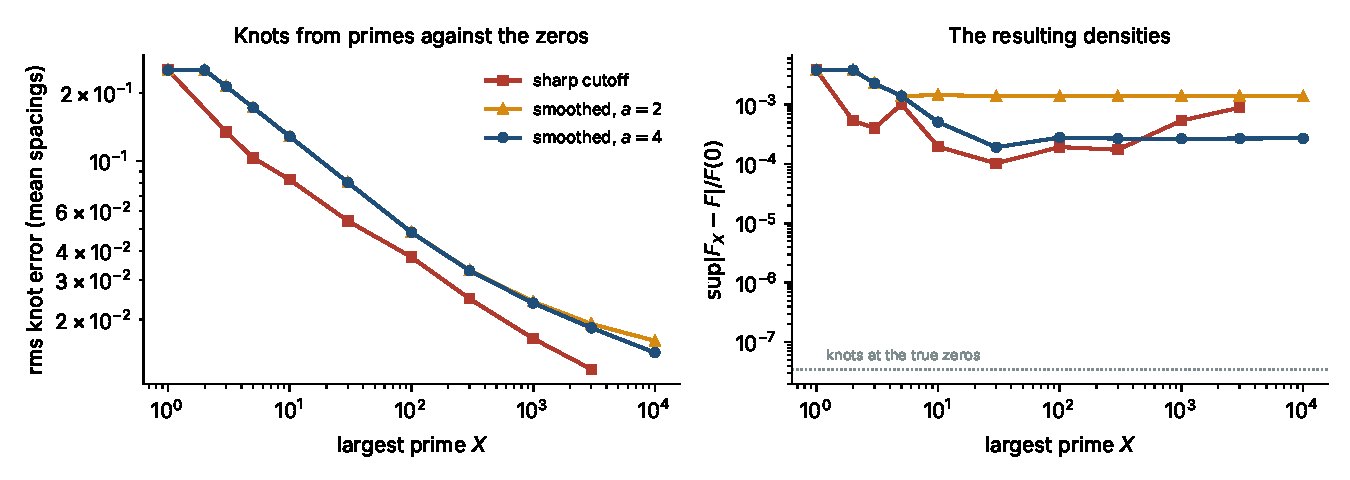
\includegraphics[width=\textwidth]{fig/v3/fig_knots.pdf}
\caption{Left: rms error of the prime knots against the zeros. Right: the error of the resulting P\'olya frequency density $F_X$ against $F$.}
\label{c:fig:knots}
\end{figure}

Table~\ref{c:tab:knots} and Figure~\ref{c:fig:knots} show three things.
\begin{itemize}
\item The knots converge on average. With smoothing the count is exactly $649$ for every $X$, and the rms error falls from $0.25$ to $0.014$ mean spacings. The primes do locate the zeros on average.
\item They do not converge at a fixed height. For fixed $t$ the sum $S_X(t)$ is independent of $X$ once $X\ge(t/2\pi)^a$, so a low knot is stationary beyond a finite cutoff: the first knot stops at $14.256$ for $a=2$ (cutoff $X\approx5$) and at $14.158$ for $a=4$ (cutoff $X\approx26$), at distances $0.12$ and $0.023$ from $\gamma_1=14.135$ (computed). The error of the density stalls near $3\times10^{-4}$, four orders of magnitude above what true knots give, because $F$ is dominated by the lowest zeros.
\item Without smoothing the construction is unstable: the truncated Euler product does not converge on the critical line, and at $X=10^4$ it creates spurious knots.
\end{itemize}
The low zeros can be computed directly to any accuracy. But then the primes act only on high knots, which barely move $F$, and the numerical comparison says nothing about them. These finite cutoff constructions produce P\'olya frequency approximants with the measured errors. To obtain $F^{\rm ord}$ one needs a different weighting and a theorem that gives convergence of the knots and a uniform tail condition.

\subsection{Why numerics cannot close the gap}

Proposition~\ref{c:prop:ord} says the missing step is $F=F^{\rm ord}$. For the control both sides can be computed, because its zeros off the line are known (Section~\ref{sec:ch21:hankel}): the lowest quadruplet is $\frac12\pm0.3085\pm85.6993\,i$, and the next is $\pm0.1508\pm114.1633\,i$ (the zero $0.6508+114.1633i$), and there are eight quadruplets below height $400$. The characteristic functions of $F^{\rm ord}_{\rm DH}$ and $F_{\rm DH}$ differ by the product over all of them of the factor $P/Q$, where each quadruplet contributes $P(\tau)=1+2(\gamma^2-d^2)\tau^2/(\gamma^2+d^2)^2+\tau^4/(\gamma^2+d^2)^2$ against $Q(\tau)=(1+\tau^2/\gamma^2)^2$. With all eight,
\[
\sup_x\big|F^{\rm ord}_{\rm DH}(x)-F_{\rm DH}(x)\big|=7.6\times10^{-8}\,F_{\rm DH}(0)\qquad(\text{computed}),
\]
attained at $x=0$. The lowest quadruplet alone gives $6.7\times10^{-8}$ and the four below height $200$ give $7.4\times10^{-8}$, so the further quadruplets change the value by $14$ per cent. The four zeros between heights $200$ and $400$ are near $0.8695+240.4047i$, $0.8195+320.8765i$, $0.7682+331.0503i$ and $0.6285+366.6409i$ (computed by a grid search in the half strip $0.52\le\beta\le2$, not certified, so that the count of eight needs a certified count).
% UNVERIFIED: the sup-norm bound of the inversion and the omission of zeros above height 400 are not bounded; the value 7.6e-8 is a double precision Simpson integral of the quadruplet factors (V7).
So there is a P\'olya frequency function within $8$ parts in $10^8$ of a density that fails rung $44$ (Section~\ref{p:sec:detect}). For $\zeta$, RH holds up to height $3\times10^{12}$ \cite{PT21}, and a zero off the line above it would make a difference smaller by many orders of magnitude. The distance from $F$ to the class of P\'olya frequency functions is zero if and only if RH holds (Proposition~\ref{c:prop:closure}, in the sense of pointwise limits), and no computation of that distance can distinguish zero from the control's $10^{-7}$. This is the detection scale of Chapter~\ref{p:ch:path} seen from the spline side.

\section{The crossing: Wald couples and the point about \texorpdfstring{$1/\xi$}{1/xi}}\label{c:sec:wald}

Proposition~\ref{c:prop:gauss} says that total positivity of every order on both sides forces the Gaussian. That is too strong a demand. The passage from $\xi$ to $1/\xi$ is a classical object, and the Gaussian is only its simplest instance.

\subsection{Three readings of \texorpdfstring{$1/\xi$}{1/xi}}

Let $X$ have density $\Phi(x)/\xi(\frac12)$, so that $\E\,e^{tX}=\xi(\frac12+t)/\xi(\frac12)$ by \eqref{c:eq:kernel}. A pair $(X,H)$ with $H\ge0$ is a Wald couple in the sense of Roynette and Yor \cite{RoynetteYor05} if
\[
\E\,e^{tX}\;\E\,e^{-t^2H/2}=1\qquad\text{for all real }t .
\]
Brownian motion run to a time $H$ has the same relation by Wald's identity, with $X$ the position, when $H$ is a stopping time for which the identity holds. In the language of Lukacs \cite{Lukacs68} the characteristic functions of $X$ and of $W=\sqrt H\,Z$, with $Z$ standard normal, form a van Dantzig pair. The link between these pairs, Thorin measures and the Hadamard product of $\xi$ is developed in \cite{P18}. In the notation of this book $H=2T$, where $T$ is the clock variable of Section~\ref{ch:clock}, so that $\E\,e^{-uT}=\xi(\frac12)/\xi(\frac12+\sqrt u)$ and the Thorin measure of $T$ is $\sum_n\delta_{\gamma_n^2}$. For $\xi$ the three readings are
\[
\frac{\xi(\frac12)}{\xi(\frac12+\tau)}\;=\;\E\,e^{i\tau W}\;=\;\E\,e^{-\tau^2H/2}\;=\;\frac1{\E\,e^{\tau X}} .
\]
The first is the Fourier transform of $F$, the second the Laplace transform of the law of $H$ at $s=\tau^2/2$, the third the reciprocal of the transform of the kernel.

\begin{proposition}\label{c:thm:wald}
\begin{enumerate}
\item The partner exists unconditionally: $T$ is infinitely divisible and self decomposable, $(\Xi(\theta)/\Xi(0),\xi(\frac12)/\xi(\frac12+\theta))$ is a van Dantzig pair and $(X/\sqrt2,T)$ is a Wald couple (Theorem~\ref{thm:ch12:idsd} and Remark~\ref{mw:rem:waldT}). Hence $F$ is a scale mixture of normals, with mixing variable $H=2T$.
\item RH holds if and only if $H$ is a generalised gamma convolution. In that case $H=\sum_n2E_n/\gamma_n^2$ with independent standard exponentials $E_n$, its Thorin measure in the variable $s$ is $\sum_n\delta_{\gamma_n^2/2}$, and, with the Krein string of Corollary~\ref{ev:cor:rh}, its density $h$ is a one sided P\'olya frequency function.
\end{enumerate}
\end{proposition}

\begin{proof}
Item 1 is Theorem~\ref{thm:ch12:idsd}, Remark~\ref{mw:rem:waldT} and Bernstein's theorem applied to $\E\,e^{i\tau W}=\E\,e^{-\tau^2H/2}$. Item 2 is Corollary~\ref{ev:cor:rh} with the change $H=2T$: under RH the Hadamard product gives $\xi(\frac12)/\xi(\frac12+\sqrt{2s})=\prod_n(1+2s/\gamma_n^2)^{-1}$, and conversely the Laplace transform of a generalised gamma convolution is $\exp(-as-\int\log(1+s/x)\,U(\mathrm dx))$, analytic and free of zeros on the plane cut along the negative axis \cite{Bondesson}, so every zero is on the line.
\end{proof}

The existence of the partner is a theorem of Volume I and not a numerical observation, and it is the reason that complete monotonicity, a single positivity condition, cannot separate $\zeta$ from a function that merely behaves like it. The question of this chapter, how to cross from $\xi$ to $1/\xi$, has the precise form: find the Wald partner of the kernel and show that it is a generalised gamma convolution. The total positivity ladder for $F$ is the same statement after mixing with the normal.

\paragraph{No wall on the side of $H$} Under RH with simple zeros the density of $H$ is
\[
h(x)=\sum_n\gamma_nc_n\,e^{-\gamma_n^2x/2},\qquad c_n=-\frac{\xi(\frac12)}{\Xi'(\gamma_n)},
\]
the same residues as in $F(x)=\sum c_ne^{-\gamma_n|x|}$. The residues grow like $e^{\pi\gamma_n/4}$, which stops the series for $F$ at $|x|=\pi/4$. Against $e^{-\gamma_n^2x/2}$ that growth is harmless: the series for $h$ converges for every $x>0$ provided $1/|\zeta'(\rho_n)|$ grows at most exponentially, an assumption that cannot be checked on finitely many zeros. The near field of $F$, where every zero acts at once, has no counterpart for $H$. Its place is taken by the limit $x\to0$, where $h$ vanishes to infinite order and the alternating terms cancel almost completely.

\subsection{Test kernels beyond the Gaussian}

For which kernels is the crossing a theorem? Whenever the transform of the kernel is of Laguerre and P\'olya form with only imaginary zeros, with a Gaussian factor of nonnegative exponent and a summable product over the zeros, the partner $H$ is a shift plus a convolution of exponentials and $W$ is a P\'olya frequency variable. Having only imaginary zeros is not enough by itself: a symmetric compound Poisson variable with jumps $\pm1$ at rate one has $\E\,e^{tX}=\exp(\cosh t-1)$, entire and free of zeros, and the candidate partner transform $\exp(1-\cosh\sqrt{2s})=1-s+s^2/3+O(s^3)$ would give $\mathrm{Var}\,H=-\frac13$. Table~\ref{c:tab:wald} lists the classical cases. In the first four the partner $H$ is a hitting time of a Bessel process started at zero (or the exit time of an interval by Brownian motion), and the zeros are those of a cosine or a Bessel function.

\begin{table}[t]
\centering
\footnotesize
\begin{tabular}{p{0.19\textwidth}p{0.19\textwidth}p{0.27\textwidth}p{0.17\textwidth}}
\toprule
law of $X$ & $\E\,e^{tX}$ & partner $H$ & law of $W$\\
\midrule
point masses at $\pm1$ & $\cosh t$ & exit time of $(-1,1)$ by Brownian motion & hyperbolic secant\\
uniform on $(-1,1)$ & $\sinh t/t$ & hitting time of $1$ by the Bessel process of dimension $3$ & logistic\\
arcsine on $(-1,1)$ & $I_0(t)$ & hitting time of $1$ by the Bessel process of dimension $2$ & $1/I_0(\tau)$\\
symmetric beta, parameter $\nu>-\frac12$ & $c_\nu t^{-\nu}I_\nu(t)$, $c_\nu=2^\nu\Gamma(\nu+1)$ & hitting time of $1$ by the Bessel process of dimension $2\nu+2$ & $1/$Bessel\\
normal & $e^{t^2/2}$ & $H=1$ & normal\\
P\'olya's kernel & Bessel $K$ sums & exponentials at P\'olya's zeros & PF function\\
Riemann's kernel & $\xi(\frac12+t)/\xi(\frac12)$ & $H=2T$, exists unconditionally, a generalised gamma convolution if and only if RH & $F$\\
\bottomrule
\end{tabular}
\caption{Wald couples. In every row but the last, the reality of the zeros is a theorem and the crossing from the kernel to the reciprocal is explicit; the dictionary between the cosine and a Brownian exit time is Table~\ref{bh:tab:dict}.}
\label{c:tab:wald}
\end{table}

These are the test functions other than the Gaussian. They show what does and does not cross.
\begin{itemize}
\item Total positivity of the kernel does not. We computed the first order $p$ at which $W_p(u)<0$ somewhere on $[0,1.5]$, for smooth kernels whose transforms are known to have only real zeros, in series arithmetic for $p\le9$ (computed, 120 digits, reproduced independently):
\begin{center}
\footnotesize
\begin{tabular}{lccccc}
\toprule
kernel & $e^{-u^2}$ & $e^{-\cosh u}$ & $e^{-u^4}$ & $e^{-u^4-u^2}$ & P\'olya 1926\\
\midrule
first negative order & none & $4$ & $5$ & $3$ & $3$\\
\bottomrule
\end{tabular}
\end{center}
For $e^{-u^4}$ the minors $W_2$ and $W_3$ vanish at $u=0$ and are positive elsewhere. P\'olya's kernel $\cosh(9u/2)\,e^{-2\pi\cosh2u}$, whose transform has only real zeros by his theorem of 1926 \cite{Polya}, fails at order $3$. Riemann's kernel fails at order $5$. So the first failing order of a kernel with real zeros ranges from $3$ to never, and says nothing about the zeros, in either direction. The point mass and uniform laws of Table~\ref{c:tab:wald} are not smooth, and the arcsine density is not even log concave, so no order is defined for them.
\item The Lee Yang property does. Call $X$ ferromagnetic if $\E\,e^{tX}$ has only imaginary zeros. This class is closed under convolution and under limits. It is closed under multiplication of the density by $e^{bu^2}$ with $b\ge0$ when the density decays faster than any Gaussian, which is de Bruijn's theorem and the forward heat flow \cite{deBruijn}, and it is not closed under sums of densities. Newman \cite{Newman1976} classified the measures that stay in the class under the backward flow, multiplication by $e^{-bu^2}$ for every $b>0$, under his decay hypotheses: they are two point masses, or densities $u^{2m}e^{-\alpha u^4-\beta u^2}\prod_j(1+u^2/a_j^2)e^{-u^2/a_j^2}$ (Section~\ref{ch:biane}). Riemann's kernel is not of that form, in agreement with $\Lambda\ge0$. P\'olya's kernel is the symmetrised leading term of Riemann's kernel, and Riemann's kernel adds the remaining terms of the sum over $n$, which is where the difficulty sits.
\end{itemize}

\subsection{The control, and what separates it}

For the control the same three readings are candidates, with $\xi_f$ in place of $\xi$ (Section~\ref{sec:ch21:hankel}). Whether the control has a partner, that is, whether its mixing density is nonnegative, has not been proved. We computed the candidate density of $H$ by numerical Laplace inversion (Talbot contours \cite{Talbot79} of degree $40$ and $56$). For $\zeta$ it is positive on $0.014\le x\le0.2$, with peak value $40$ near $x=0.04$. For the control it is positive on $0.02\le x\le1$, with peak $6.7$ near $x=0.15$; a second run in $110$ digit arithmetic with contours of degree $90$ and $110$ resolves values down to $10^{-41}$ and gives $2.1\times10^{-29}$ at $x=0.02$ (computed). Below these ranges the densities are smaller than the resolution of the inversion. There the transform is governed by the gamma factor, as for a genuine $L$ function, and no sign change is expected. So to thirty orders of magnitude the computed density of the control is positive, which is consistent with a scale mixture of normals and does not prove it.
% UNVERIFIED: the Talbot inversion densities (positive ranges, peaks 40 and 6.7, 2.1e-29) are the draft's; the verification (V18) did not rerun them. They are given in the variable of H = 2T.

What separates the control is the second half of Proposition~\ref{c:thm:wald}. Its partner cannot be a generalised gamma convolution, because its Thorin measure would need the complex atoms $-(\pm0.3085+85.6993\,i)^2$ in the variable $u$ of $T$, which have real part $+7344$. Existence of $H$ is complete monotonicity, a single positivity condition that the control appears to satisfy. That $H$ is a generalised gamma convolution is positivity of the Thorin measure, and for $\zeta$ that is RH.

\section{Two more ladders, from real axis data}\label{c:sec:grommer}

Proposition~\ref{c:thm:wald} turns into finite inequalities that use only the Taylor coefficients of $\log\xi$ at $\frac12$, with no zeros as input. For each pair of zeros $\rho=\frac12\pm w$ put $b=-1/w^2$, so that $b=1/\gamma^2>0$ for a zero on the line. Let
\[
p_k=\sum b^k=-k(-1)^k\,[\tau^{2k}]\log\frac{\xi(\frac12+\tau)}{\xi(\frac12)},\qquad k\ge1,
\]
so that $\E\,e^{-uT}=\exp\big(\sum_k(-1)^kp_ku^k/k\big)$, the $p_k$ are the moments of the Thorin measure in the variable $b=1/\gamma^2$, and the moments $\E\,T^k$ follow from the exponential series. In the notation of Section~\ref{sec:ch21:hankel} and Theorem~\ref{thm:ch12:inertia}, $m_n=p_{n+1}$, and $\mathcal H_N=[m_{i+j}]_{i,j<N}$, $\mathcal H'_N=[m_{i+j+1}]_{i,j<N}$ are the Hankel matrices of the measure $\nu=\sum b_n\delta_{b_n}$. The two ladders are the determinants $D_N=\det\mathcal H_N$ and $D'_N=\det\mathcal H'_N$.

\begin{proposition}\label{c:prop:grommer}
\begin{enumerate}
\item (Thorin ladder.) RH holds if and only if $D_N>0$ and $D'_N>0$ for every $N\ge1$.
\item (Moment ladder.) For every $N\ge1$, $M_N=\det[\E\,T^{i+j}]_{i,j<N}>0$ and $M'_N=\det[\E\,T^{i+j+1}]_{i,j<N}$ are positive.
\end{enumerate}
\end{proposition}

\begin{proof}
Item 1 is Grommer's criterion \cite{Grommer14} in the present variables, and Theorem~\ref{thm:ch12:inertia} is stronger, since the inertia of $\mathcal H_N$ counts the zeros off the line. For a proof of the direction used here: under RH, $\nu$ is a positive measure on $(0,\infty)$ with infinitely many atoms, and by the Cauchy Binet formula $D_N=\sum_{|S|=N}\prod_{i\in S}b_i\prod_{i<j}(b_i-b_j)^2>0$, and likewise $D'_N>0$. Conversely, strict positivity of all the leading minors makes every $\mathcal H_N$ and $\mathcal H_N'$ positive definite (Sylvester), so by Stieltjes's theorem there is a positive measure $\nu'$ on $[0,\infty)$ with moments $m_{k}$ and $m_{k+1}$ against $1$ and $x$. Weak inequalities would not suffice: the four fourth roots $b$ of $-1$ have power sums with $D_N,D'_N\ge0$ for every $N$ and fourth power sum $-4$, so that no positive measure has these moments. Since $|p_k|\le Cr^k$ the measure has bounded support, and $\sum_km_kz^k=\int\nu'(\mathrm da)/(1-az)$ is analytic off the positive real axis. The same series equals $\sum_nb_n/(1-b_nz)$, with poles at the points $1/b_n$, and the residue at each distinct pole is a positive multiple of the multiplicity of the zero. So every $b_n$ is real and positive, every $w_n^2$ is negative, and RH holds.

For item 2, the law of $T$ has infinite support: if it were finitely supported then $1/G$ would be a finite exponential sum without zeros in the whole plane, hence a single exponential, which contradicts the order $\frac12$ of $G$ and its zeros. So every nonzero polynomial has positive squared integral against the law of $T$ and against the law weighted by $T$, which is the strict positivity.
\end{proof}

We computed the Thorin ladder for $\zeta$ and for the control, to $N=50$, from Taylor series of the kernel moments, in ball arithmetic with $38000$ bit floating point input: the balls are rounding balls of the determinants, so every sign below is computed and not certified. All $D_N$ and $D'_N$, $N\le50$, are positive.

\begin{center}
\footnotesize
\begin{tabular}{rcccc}
\toprule
 & \multicolumn{2}{c}{$\zeta$} & \multicolumn{2}{c}{control}\\
$N$ & $D_N$ & $D_N'$ & $D_N$ & $D_N'$\\
\midrule
$10$ & $1.01\times10^{-299}$ & $6.63\times10^{-333}$ & $8.03\times10^{-230}$ & $1.85\times10^{-256}$\\
$20$ & $9.53\times10^{-1326}$ & $7.56\times10^{-1398}$ & $1.00\times10^{-1077}$ & $1.66\times10^{-1138}$\\
$30$ & $2.50\times10^{-3158}$ & $3.78\times10^{-3272}$ & $5.94\times10^{-2641}$ & $4.50\times10^{-2739}$\\
$40$ & $1.38\times10^{-5843}$ & $5.04\times10^{-6001}$ & $2.73\times10^{-4972}$ & $6.08\times10^{-5110}$\\
$50$ & $1.86\times10^{-9415}$ & $5.79\times10^{-9618}$ & $2.89\times10^{-8110}$ & $4.22\times10^{-8289}$\\
\bottomrule
\end{tabular}
\end{center}
The control is the function $\xi_f$ of Section~\ref{sec:ch21:hankel}, and its first coefficients agree with that section. The moment ladder $M_N$, $M'_N$ was reported positive for both functions to $N=50$ in the note and is not recomputed here. Three conclusions follow.
% UNVERIFIED: the moment ladder M_N, M_N' to N=50 for zeta and the control (V6 did not recompute them).
\begin{itemize}
\item For $\zeta$ the first $50$ rungs of the Thorin ladder hold, by a computation that never locates a zero. For $\zeta$ Section~\ref{sec:ch21:hankel} reports more, $c_1,\dots,c_{1299}>0$ from the Taylor coefficients, from an unrefereed note of Polson, recomputed there to $c_{519}$ in floating point.
\item The control passes the moment ladder, as it must if it has a Wald partner, and together with the positive mixing density above this is evidence, not proof, that the control has one, so that complete monotonicity does not separate it from $\zeta$.
\item The control also passes the first $50$ rungs of the Thorin ladder, although it fails the P\'olya frequency ladder of $F$ at rung $44$. The Thorin ladder must fail for the control at some $N$, by Proposition~\ref{c:prop:grommer}, but it is the blunter instrument. The reason is visible in the Cauchy Binet sum. The quadruplet off the line gives the conjugate atoms $b_*=x\pm iy$ with $x=1.36\times10^{-4}$ and $y/x\approx0.0072$, and it enters with a negative sign only through $(b_*-\bar b_*)^2=-4y^2$, which is small against the squared distance to the neighbouring atoms. To the Hankel determinants the pair looks like a double real atom until $N$ is large enough for that factor to matter. In the ladder of $F$ the same pair is amplified by the free shift $L$, through $\cos(dL+\theta)$.
\end{itemize}

\paragraph{Where the Thorin ladder fails for the control} The failing rung can be estimated from the zeros, and the estimate is the Christoffel function method of Proposition~\ref{prop:ch21:verhankel} applied to the control. $D_N$ is the determinant of the form $p\mapsto\sum_kb_k\,p(b_k)^2$ on polynomials of degree below $N$, and $D'_N$ that of $p\mapsto\sum_kb_k^2\,p(b_k)^2$. Take $p(t)=(t-x)q(t)$ with $q$ real. The conjugate pair then contributes $2\re[b_*p(b_*)^2]\approx-2xy^2q(x)^2$, and the real atoms contribute $\sum_kb_k(b_k-x)^2q(b_k)^2$. So the form takes a negative value as soon as
\begin{gather*}
\lambda_d(x)<2xy^2=2.6\times10^{-16},\\
\lambda_d(x)=\min\Big\{\sum_kb_k(b_k-x)^2q(b_k)^2:\ \deg q\le d,\ q(x)=1\Big\},
\end{gather*}
and $\lambda_d(x)$ is the Christoffel function of the positive measure $\sum_kb_k(b_k-x)^2\delta_{b_k}$, which decreases to zero as $d$ grows. We located the $287$ real zeros of the control below height $400$ and computed $\lambda_d(x)$ by the Stieltjes procedure in $600$ digit arithmetic. The first degree below the threshold is $d=66$, $71$ and $72$ when the zeros are cut off at heights $150$, $250$ and $400$, and $73$ when the zeros above $400$ are added as a single atom at the origin (computed). With $N=d+2$ this puts the first failing rung of the Thorin ladder near
\[
N\approx75 ,
\]
against $44$ for the ladder of $F$ and consistent with the positivity to $N=50$. The estimate ignores the other quadruplets off the line below height $400$, replaces $q(b_*)$ by $q(x)$ and moves a tail to the origin, so it is an estimate and not a bound; the threshold $2xy^2$ is for the simplified model. It is confirmed by the direct computation of Section~\ref{sec:ch21:hankel} and Chapter~\ref{b:ch:chain}: the Stieltjes coefficients $c_1,\dots,c_{147}$ of the control are positive and $c_{148}$ is negative, floating point at high precision, and $\mathcal H_{75}$ and $\mathcal H'_{75}$ are not positive definite. So among the three ladders the P\'olya frequency ladder of $F$ detects a zero off the line first, the Thorin ladder later, and the moment ladder not in the range computed.
% UNVERIFIED: the Christoffel estimate (d = 66, 71, 72, 73; 287 real zeros below 400) is the draft's; V6 did not rerun it. The threshold 2xy^2 = 2.6e-16 is the draft's 2.1e-15 divided by 8 (the conversion to the variable b = a/2), and 2xy^2 was recomputed from the zero 0.8085171825+85.6993484854 i.

\subsection{The Thorin string}\label{c:sec:string}
% Figure fig_string.pdf of the draft (alpha_n of zeta and the control against the Brownian values) is NOT included: it plots the draft's rates alpha_n = 2 c_n and must be redrawn with the halved rates c_n (Brownian values 1/(4n^2-1)) before use.

The verdict of this chapter asks for the Wald partner $H$ as a hitting time of a string built from the primes. The object that can be computed from real axis data is the Stieltjes continued fraction of $G'/G$, with $G(u)=\xi(\frac12+\sqrt u)/\xi(\frac12)$, which is the birth and death chain of Chapter~\ref{b:ch:chain}. This section reaches it from the Wald couple, and its coefficients agree with those of Section~\ref{sec:ch21:hankel} and of that chapter. Let
\[
\frac{G'}G(u)=\sum_n\frac{b_n}{1+b_nu}=\sum_{k\ge0}(-1)^kp_{k+1}u^k=\cfrac{m_0}{1+\cfrac{c_1u}{1+\cfrac{c_2u}{1+\cdots}}},
\]
\[
c_{2n-1}=\frac{D_{n-1}D_n'}{D_nD_{n-1}'},\qquad c_{2n}=\frac{D_{n+1}D_{n-1}'}{D_nD_n'},\qquad D_0=D'_0=1,
\]
where $m_0=p_1=\sum_n\gamma_n^{-2}=0.02310$.

\begin{proposition}\label{c:prop:string}
Suppose all the determinants $D_N,D'_N$ are nonzero, so that the coefficients are defined. Then RH holds if and only if $c_n>0$ for every $n$. Under RH, $G'/G$ is a Stieltjes function whose measure is the Thorin measure $\sum_n\delta_{\gamma_n^2}$, hence the principal Weyl function of a unique Krein string, and the string of the hitting time of Corollary~\ref{ev:cor:rh}.
\end{proposition}

\begin{proof}
Stieltjes's theorem: the continued fraction has positive coefficients if and only if the $m_k$ are the moments of a positive measure on $(0,\infty)$ with infinite support, which by Proposition~\ref{c:prop:grommer} is RH. Under RH the identity $G'/G=\int\nu(\mathrm db)/(1+bu)$ with $\nu=\sum_nb_n\delta_{b_n}$, and the substitution $b=1/\lambda$, give the Thorin measure $\sum_n\delta_{\gamma_n^2}$, and the string is Krein's inverse spectral theorem \cite{KacKrein74}.
\end{proof}

A positive string exists if and only if RH holds: without RH there is only a formal continued fraction. The coefficients $c_n$ are the parameters of the fraction, not the masses and gaps of the string, which are obtained from them after the change $b=1/\lambda$ of the spectral parameter, and the string of a continuous Brownian segment is not a sequence of point masses. The test case is the first row of Table~\ref{c:tab:wald}. For $\E\,e^{tX}=\cosh t$ one has $G=\cosh\sqrt u$, $G'/G=\frac12\tanh\sqrt u/\sqrt u$, and Lambert's continued fraction gives
\[
c_n=\frac1{(2n-1)(2n+1)},
\]
the string of Brownian motion on an interval. For $\xi$ we computed $c_1,\dots,c_{98}$ from the determinants above, positive (computed):
\begin{gather*}
c_1=0.0016089,\quad c_2=0.0022696,\quad c_3=0.0012309,\\
c_4=0.0010733,\ \dots,\ c_{98}=3.06\times10^{-5},
\end{gather*}
and for the control $c_1=0.01783$, $c_2=0.01631$, $c_3=0.00683$, $c_4=0.00568$ and $c_{98}=6.4\times10^{-5}$, positive to $c_{98}$, with the negative values at $c_{148}$ (Section~\ref{sec:ch21:hankel}) and $c_{150}$ (Chapter~\ref{b:ch:chain}).

The string is a Brownian string with a local change of scale. For the cosine the atoms are $b_m=1/(\pi^2(m-\frac12)^2)$ and $c_n\approx\frac{\pi^2}{16}b_{n/2}$. For $\xi$ the same rule with the true ordinates holds up to a slowly varying factor,
\[
c_n=\rho_n\,\frac{\pi^2}{16\,\gamma_{\lceil n/2\rceil}^2},\qquad\rho_n=0.89\pm0.06\quad(20\le n\le98)\qquad(\text{computed}),
\]
and for the control $\rho_n=0.92\pm0.07$ in the same range (computed), with no mark of its pair off the line there; the mark is at $c_{148}$ and $c_{150}$, the level where the turning height of the preceding positive rates reaches the ordinate $85.7$. This is the bluntness of the Thorin ladder again. The local comparison carries a fitted constant. The law \eqref{eq:ch21:ratelaw} of Section~\ref{sec:ch21:hankel} has none and describes the same main term (heuristic); the model below only checks it locally.
% UNVERIFIED: rho_n = 0.92 +- 0.07 and the control slope 0.77 below are the draft's (V6 did not run the rho statistics). The zeta value rho = 0.89 +- 0.06 and the slope 0.66 were reproduced independently (0.8895, 0.0599; 0.6575).

\paragraph{Where the factor $0.89$ comes from} Take model atoms $b_n=1/\gamma_n^2$ with $\gamma_n=\pi(n-\frac12)^\beta$, $\beta>\frac12$, so that $\beta=1$ is the cosine. Their moments are $p_k=\pi^{-2k}(2^{2\beta k}-1)\zeta(2\beta k)$, and the Stieltjes coefficients follow as before. The ratio $\rho_n$ settles quickly:
\begin{center}
\footnotesize
\begin{tabular}{rcccccc}
\toprule
$\beta$ & $1$ & $0.9$ & $0.8$ & $0.7$ & $0.66$ & $0.6$\\
\midrule
$\rho_{78}$ & $0.975$ & $0.951$ & $0.925$ & $0.895$ & $0.881$ & $0.860$\\
\bottomrule
\end{tabular}
\end{center}
with $\rho_n\to1$ for $\beta=1$ (proved, from Lambert's fraction), and the values for the other $\beta$ at $n=78$ computed. The zeros of $\zeta$ in the computed range grow like $\gamma_m\propto m^{0.66}$ (the slope of $\log\gamma_m$ against $\log m$ for $10\le m\le49$), and the model with $\beta=0.66$ gives $\rho=0.88$, against the observed $0.89$. For the control the slope is $0.77$ and the model gives about $0.92$, the observed value. So the main term is fixed by the local growth exponent of the ordinates, that is by the gamma factor, and since the exponent tends to $1$ with height one expects $\rho_n\to1$ slowly. The law \eqref{eq:ch21:ratelaw} gives the same main term for the block means of the rates with no fitted constant, checked there to $0.2$ per cent up to $j=1299$ (heuristic), and the model of this paragraph is a weaker, local version of it. What the model does not give is the fluctuation: it is $0.06$ for $\zeta$ and below $0.005$ for the model. The correlation of $\log\rho_{2m}$ with the normalised spacing around the $m$th zero is only $-0.24$ (computed).

\paragraph{Separating the arithmetic} The coefficients can also be computed from a list of ordinates, by the discrete Stieltjes procedure for the measure $\sum b_k\delta_{b_k}$ with the ordinates above the list lumped at the origin. With the first $9000$ zeros this reproduces the $c_n$, $n\le98$, to within $0.4$ per cent (computed). Applied to the smooth ordinates $g_m$ of Section~\ref{c:sec:knots}, which use the gamma factor only, it gives
\begin{gather*}
\rho_n^{\rm smooth}=0.889\pm0.016,\qquad\rho_n^{\rm true}=0.890\pm0.060,\\
\frac{c_n^{\rm true}}{c_n^{\rm smooth}}=1.001\pm0.067\qquad(20\le n\le98),
\end{gather*}
with the last ratio between $0.88$ and $1.15$ (computed). The mean is the same to three digits over this range, which is evidence that the main term is the gamma factor and that the arithmetic is a multiplicative fluctuation of about seven per cent around the smooth string, in the range computed. We do not claim that the main term is exact or that the fluctuation is bounded: the asymptotic form is open. The fluctuation is the displacement of the zeros from the points $g_m$, which to first order is $-\pi S(t)/\theta'(g_m)$ with $S(t)=\frac1\pi\arg\zeta(\frac12+it)$ the Euler product correction of Section~\ref{c:sec:knots}, and through it the primes.
% UNVERIFIED: the smooth ordinate comparison (0.889 +- 0.016, 1.001 +- 0.067, the 0.4 per cent from 9000 zeros) is the draft's; the verification did not run it.

\section{What the two candidates leave}\label{c:sec:verdict}

Neither candidate is a mechanism in the sense of Milestone Four of Chapter~\ref{p:ch:path} (Section~\ref{p:sec:milestones}), and each failure leaves a sharper requirement. From candidate one: the arithmetic gives total positivity on the kernel side, where it cannot be complete and where it does not track the zeros, since the control and $L(s,\chi_4)$ stop at the same rung. The crossing from $\xi$ to $1/\xi$ is the Wald couple, and what crosses is the Lee Yang property. The test kernels of Table~\ref{c:tab:wald} cross because their transforms are cosines and Bessel functions with a product structure over zeros. For $\xi$ the product structure is over primes, on the wrong side. From candidate two: constructing P\'olya frequency approximants is easy and proves nothing, because the ordinates of zeros always supply one. A mechanism must compare with the real axis data, that is, prove $F=F^{\rm ord}$, and it must do so by an identity, since the two sides can agree to $10^{-7}$ and differ. The prime knots computed here are finite cutoff approximants with measured errors and do not deliver $F^{\rm ord}$.

From the Wald couple: the target can be moved from $F$ to its mixing variable $H$, where there is no wall at $\pi/4$ and where RH is the positivity of a Thorin measure. That positivity has its own ladder, computable from real axis data, of which $\zeta$ passes the first $50$ rungs, but the control passes them too, so the ladder of $F$ remains the sharper test. A partner $H$ that is a hitting time of a diffusion built from the primes would be a mechanism. Every classical example in Table~\ref{c:tab:wald} has that form, in the boundary to boundary version of the Brownian row (a hitting time of a reflected diffusion need not be a convolution of exponentials \cite{Kent80}). For $\xi$ the Stieltjes fraction exists as a formal object and its first $98$ coefficients are computed and positive (Section~\ref{c:sec:string}); what is missing is a formula for them that is visibly positive, as $1/(4n^2-1)$ is. The path of Chapter~\ref{p:ch:path} is unchanged by this chapter: two side roads are closed, and one is reopened in a sharper form, to find a positive formula for the Stieltjes coefficients of $\xi$.

The open problems are the following.
\begin{enumerate}
\item Explain why the kernel of $\zeta$ climbs higher than the kernels of the Dirichlet $L$ functions tested. Is the first failing rung of the kernel related to the conductor, to the height of the lowest zero, or to the Euler product? The characters modulo $3$ and $4$, both odd, have orders $3$ and $2$.
\item The local form. The failure of $\Phi$ at order $5$ is a sign condition on derivatives of $\Phi$ at the origin. Express it through the moments of $\Phi$, that is, the Taylor coefficients of $\xi$ at $\frac12$, and compare with the Tur\'an and Laguerre inequalities, which are conditions on the same coefficients.
\item The heat flow on the kernel side. The local order of $e^{tu^2/4}\Phi$ at the origin grows as $t\to-\infty$ and falls as $t\to\infty$. Is there a law linking it to the failing rung $r(t)$ of the density $F_t$? No simple one: for $-5\le t\le0$ the local order of the kernel stays at $5$ while the bound on $r(t)$ rises from $4$ to infinity, the value at $t=0$ only under RH.
\item Make Propositions~\ref{c:thm:tp4} and \ref{c:thm:lk} theorems, by a rigorous enclosure of $W_p/K^p$ over the window and the tail, and say what governs the order of the kernel of a primitive $L$ function.
\item The control's mixing density. Is the inverse Laplace transform of $\xi_f(\frac12)/\xi_f(\frac12+\sqrt{2s})$ nonnegative? The density is positive where it can be resolved. A proof would show that complete monotonicity is strictly weaker than RH for this family.
\item The failing rung of the Thorin ladder for the control, and the law of the rates $c_j$ of $\xi$, are treated in Section~\ref{sec:ch21:hankel} (the rung near $75$ and \eqref{eq:ch21:ratelaw}). What remains open there is a theorem for the estimate, and the explicit formula for the fluctuation $c_n^{\rm true}/c_n^{\rm smooth}$, which is the arithmetic part: to first order a linear functional of $S(t)$ at the low ordinates.
\item A hitting time for $\xi$. Is $H$ the hitting time of a diffusion whose speed measure is built from the primes? Kent's theorem \cite{Kent80} makes every hitting time of a diffusion on an interval, from boundary to boundary, a convolution of exponentials, and the Thorin string is one candidate for the underlying string.
\item A duality between the two ladders. Is there an inequality linking the order of total positivity of a kernel $K$ and that of the density with characteristic function $M(0)/M(\tau)$? The Gaussian is the only case where both are infinite.
\item Prime knots at low height. Find a weighting of the primes for which the first knot converges to $\gamma_1$. The smoothed sums here stall at distance $0.02$ and $0.12$.
\item A lower bound for the distance from the control's density to the P\'olya frequency class, from its negative minor of order $44$. This would calibrate what accuracy a comparison of $F$ with $F^{\rm ord}$ needs.
\end{enumerate}
